% REFERENCIAL TEORICO----------------------------------------------------

\chapter{REFERENCIAL TEÓRICO}
\label{chap:referencialTeorico}

\section{TECNOLOGIA NA PESCA}
\label{sec:referenciasDeDesenvolvimento}

\citeonline{de2022roraima} destaca que a pesca surgiu como uma prática adotada pelos seres humanos para obter alimento. Com o passar do tempo, essa atividade tornou-se mais eficiente, graças ao desenvolvimento de diversas técnicas de pesca e à utilização de iscas variadas, o que aprimorou a captura dos peixes.

Devido satisfação proporcionada pela captura de peixes, a pesca passou a ser uma atividade recreativa para muitas pessoas, o que eventualmente a transformou em um esporte. Nesse contexto, pescadores competem para capturar o maior peixe ou a maior quantidade possível, tornando a prática uma verdadeira competição.

Diante do avanço tecnológico, diversos modos de aperfeiçoar as formas de captura foram criadas, como dispositivos de localização, sonares, melhores apetrechos de pesca, e entre outras tecnologias.

Com o objetivo de aumentar a eficiência na busca por bons locais de pesca, este projeto visa criar um aplicativo que utilize a internet para permitir que pescadores compartilhem suas localizações e capturas. Dessa forma, os usuários poderão acessar informações diversas sobre as espécies capturadas, otimizando suas experiências e promovendo a troca de conhecimentos entre a comunidade de pescadores.

\section{PRODUTOS SEMELHANTES}
\label{sec:referenciasDeDesenvolvimento}

Produtos que procuram ou possuem a mesma finalidade esperada por este projeto existem, entre eles se destacam dois: O aplicativo móvel FishAngler - \textit{Fishing App}, e a ferramenta FishFriender. O aplicativo FishAngler possui muitos recursos para auxiliar os pescadores, tal como um mapa para localização e gerenciamento de pontos de pesca, descrição detalhada sobre o clima, registros de equipamentos, registro de peixes, e entre outras funcionalidades.

Um dos principais recursos disponibilizados pela ferramenta está sendo apresentado na Figura \ref{fig:fishAnglerApp}, contando com mapa localizado na atual região do usuário e diferentes tipos de ponto de referência, os quais apontam a alguma pesca ou peixe capturado.

\begin{figure}[H]
    \centering
    \caption{FishAngler - Aplicativo móvel de pesca}
    \label{fig:fishAnglerApp}
    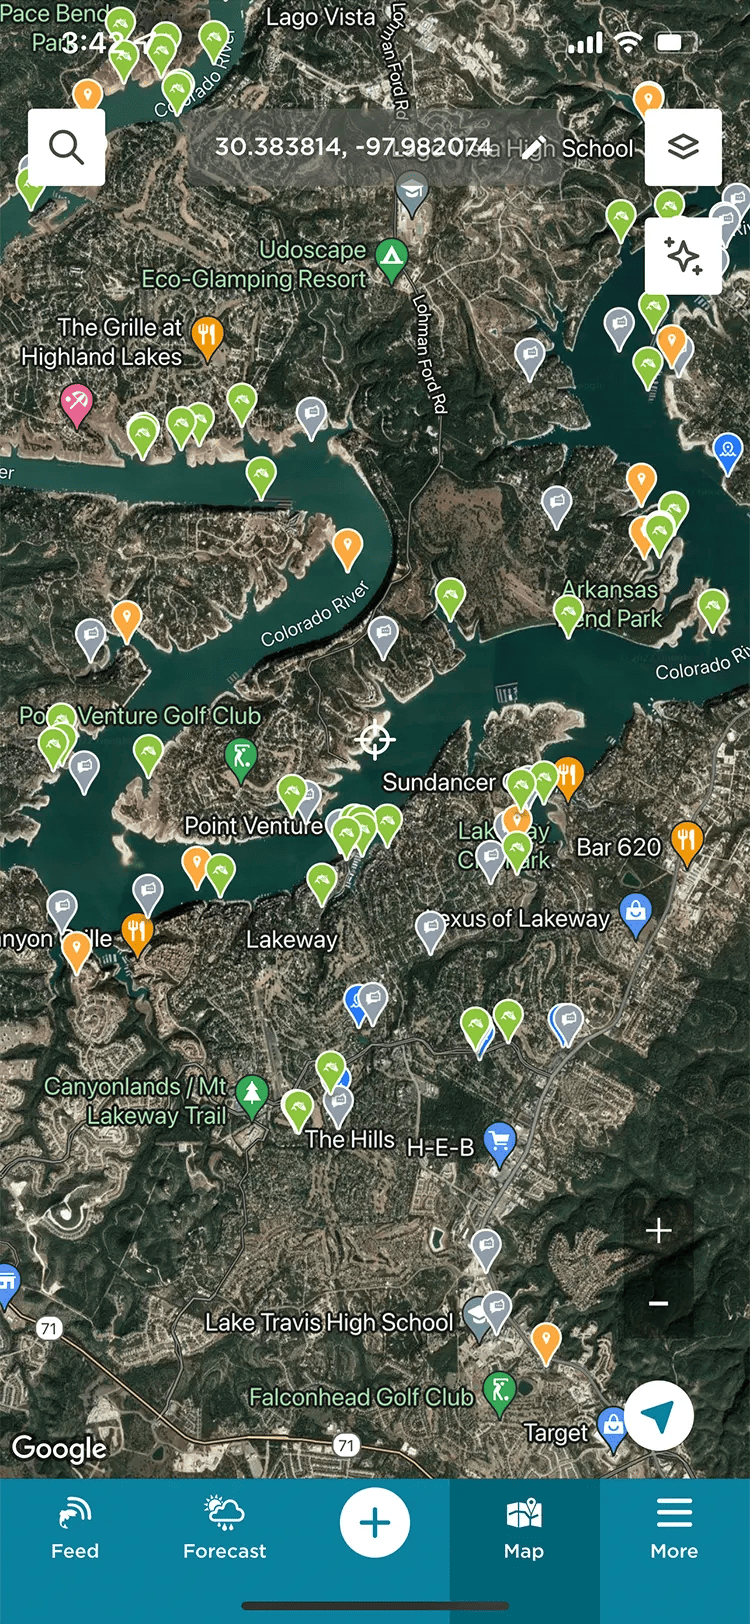
\includegraphics[scale=0.25]{./dados/figuras/fish-angler-app-map}
    \fonte{\citeonline{FishAngler24}}
\end{figure}

Apesar deste aplicativo possuir muitas funcionalidades e recursos, este não conta com a tradução para o português, resultando em uma baixa adesão por parte dos brasileiros, em sua maioria, não familiarizados com a língua inglesa.

O outro produto, FishFriender, que também possui funcionalidades semelhantes ao esperado para este projeto. A ferramenta conta com um aplicativo móvel e também uma página \textit{Web}. O aplicativo dispõe de funcionalidades como registrar peixes, registrar sessões de pesca e a possibilidade de compartilhar as informações com outros usuários.

A principal página do aplicativo móvel está sendo apresentada na Figura \ref{fig:fishFrienderApp}, esta conta com as principais capturas, os melhores contribuidores, propagandas, avisos e entre outras informações relacionadas às capturadas compartilhadas pelos usuários.

\begin{figure}[H]
    \centering
    \caption{FishFriender - Diario de pesca}
    \label{fig:fishFrienderApp}
    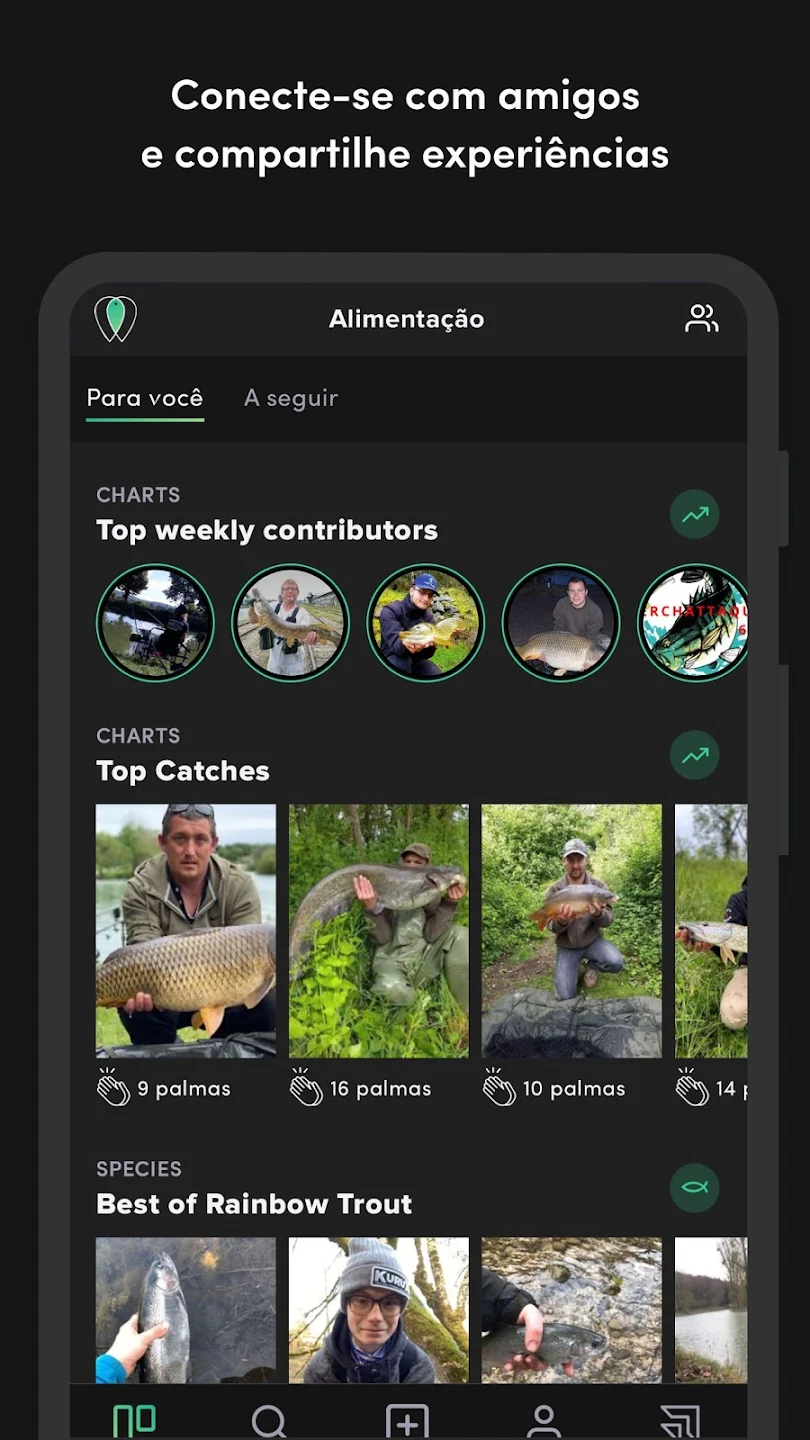
\includegraphics[scale=0.25]{./dados/figuras/fish-friender-app-feed}
    \fonte{\citeonline{FishFrienderPlayStore24}}
\end{figure}

Embora o aplicativo móvel ofereça diversas funcionalidades e recursos, ele não possui completa tradução para o português, acarretando problema similar do produto já citado neste documento.

\section{FERRAMENTAS E TECNOLOGIAS}
\label{sec:feramentasETecnologias}

As ferramentas, tecnologias e ambientes de desenvolvimento que serão utilizados no processo de desenvolvimento deste projeto são de \textit{open source} (código-fonte) ou possuem sua versão para a comunidade onde não é permitido o uso comercial ou empresarial. Segundo \citeonline{ferreira2005open} tecnologias open source são aquelas onde todos podem ter livre acesso para qualquer fim.

Para a criação da \textit{Application programming interface} (API) foi escolhido a plataforma de desenvolvimento .NET, esta conta com a linguagem de programação C\#, além de possuir diversas funcionalidades e recursos que facilitam o desenvolvimento de aplicativos, jogos, e entre outras ferramentas, como tratado pela documentação oficial da \citeonline{Microsoft24}.

O conjunto de bibliotecas Flutter foi escolhido para criar a aplicação móvel, a página web oficial do \citeonline{FlutterWeb24} descreve que o \textit{framework} utiliza a linguagem de programação multiplataforma Dart, e tem como premissa atender usuários de diversas plataformas com apenas um código-fonte.

Visual Studio e Visual Studio Code serão os ambientes de desenvolvimento  utilizados durante o processo de desenvolvimento. O Visual Studio Code conta com sua versão de código aberto, livre de restrições comerciais ou monetárias; o Visual Studio possui sua versão comunitária onde o uso é restrito para fins educacionais.

\section{PERSISTÊNCIA DE DADOS}
\label{sec:persistenciaDeDados}

Para a persistência dos dados será utilizado o banco de dados não relacional orientado a documentos MongoDB, escolha feita devido à sua alta flexibilidade com gerenciamento de dados. O MongoDB conta com seu armazenamento utilizando objetos \textit{JavaScript Object Notation} (JSON), tornando mais fácil incluir novas propriedades, criar novas relações, entre outras possibilidades. 

Segundo a página do \citeonline{MongoDB24}, a plataforma conta com diversos recursos que podem auxiliar o desenvolvedor a gerenciar e estruturar os dados com mais agilidade. O MongoDB Compass ambiente utilizado para gerenciar conexões e dados, é um dos recursos proporcionados pela plataforma e será utilizado durante o desenvolvimento do projeto.

